\section{Zielsetzung}
\label{sec:Zielsetzung}
In diesem Versuch soll die Schallgeschwindigkeit in Acryl mithilfe des Impuls-Echo Verfahren bestimmt werden.
Zusätzlich wird mit derselben Methode ein Acrylblock auf Fehlstellen, sowie ein Augenmodell untersucht.

\section{Theorie}
\label{sec:Theorie}

\subsection{Die allgemeine Schallwelle}
\label{Schallwelle}

Der Schall ist eine longitudinale Welle und kann wie folgt beschrieben werden:
\begin{equation*}
    p(x, t) = p_0 + v_0 \cdot Z \cdot \cos(\omega \cdot t - k \cdot x).
\end{equation*}
Dabei ist $Z = c \cdot \rho$ die akustische Impedanz, auch Schallkennwiderstand genannt.
$\rho$ beschreibt die Dichte des durchstrahlten Materials, $c$ die Schallgeschwindigkeit in diesem Material.

\noindent
Die Phasengeschwindigkeit einer Schallwelle ist materialabhängig.
In Flüssigkeiten hängt sie neben der Dichte $\rho$ auch von der Kompressibilität $\kappa$ ab.
Es gilt:
\begin{equation*}
    c_\text{Fl} = \sqrt{\frac{1}{\kappa \cdot \rho}}.
\end{equation*}
Wird die Schallwelle in einem Festkörper betrachtet, kommt aufgrund von Schubspannungen ein transversaler Anteil zur Welle hinzu.
In diesem Fall wird das Elastizitätsmodul $E$ hinzugezogen um die Schallgeschwindigkeit auszudrücken:
\begin{equation*}
    c_\text{Fe} = \sqrt{\frac{E}{\rho}}.
\end{equation*}
Zusätzlich ist die Schallgeschwindigkeit in Festkörpern richtungsabhängig und unterscheidet sich somit für den longitudinalen
und transversalen Anteil der Welle.

\noindent
Ähnlich wie die elektromagnetische Welle kann die Schallwelle reflektiert oder gebrochen werden.
Unteranderem wird ein Teil der Energie bei Ausbreitung der Welle absorbiert.
Für die Abnahme der Intensität $I_0$ über die Strecke $x$ gilt:
\begin{equation} \label{eqn:absorptionkoeff}
    I(x) = I_0 \cdot \symup{e}^{-\alpha \cdot x}.
\end{equation}
Hier ist $\alpha$ der Absorptionskoeffizient.
Bei Auftreffen der Welle auf eine Grenzfläche wird ein Teil reflektiert.
Dieser Reflexionskoeffzient kann dann über die akustischen Impedanzen $Z$ der beiden Materialen ausgedrückt werden:
\begin{equation*}
    R = \biggl(\frac{Z_1 - Z_2}{Z_1 + Z_2}\biggr)^2.
\end{equation*}
Der Transmissionskoeffizient $T$ folgt aus $T = 1 - R$.

\subsection{Der Ultraschall}
\label{subsec:ultraschall}

Schallwellen werden nach bestimmten Frequenzbereichen kategorisiert.
Während der Mensch Frequenzen von $\SI{16}{\hertz}$ bis $\SI{20}{\kilo\hertz}$ wahrnimmt, 
werden Frequenzen über $\SI{20}{\kilo\hertz}$ bis zu $\SI{1}{\giga\hertz}$ als Ultraschall bezeichnet.

\noindent
Um diesen Ultraschall zu erzeugen, wird der reziproken piezo-elektrischer Effekt verwendet.
Hierbei wird ein piezoelektrischer Kristall in einem elektrischen Wechelfeld zum Schwingen angeregt, wodurch Ultraschallwellen entstehen.
Bei Resonanz können besonders große Schwingungsamplituden erzeugt werden, diese erlauben eine Nutzung von hohen Schallenergiedichten.
Der Kristall kann auch als Schallempfänger verwendet werden. Dabei wird der Kristall durch die auftreffenden Schallwellen zum Schwingen angeregt.
Der meist benutzte piezoelektrischer Kristall ist Quarz, aufgrund seiner stabilen physikalischen Eigenschaften.
Nur ist der piezoelektrischer Effekt bei Quarz relativ schwach.

\noindent
Um einen Körper mithilfe von Ultraschall zu untersuchen, werden häufig Laufzeitmessungen durchgeführt.
Ein kurzer Schallimpuls wird ausgesendet und von einem Empfänger aufgenommen.
Die dafür benötigte Laufzeit wird dabei gemessen,  die zurückzulegende Strecke wird zuvor definiert.
Dazu gibt es zwei Verfahren in der Ultraschalltechnik: das Durchschallungs- und das Impuls-Echo-Verfahren.

\subsubsection{Das Durchschallungsverfahren}
\label{subsubsec:durchschall}
An einem Körper befindet sich auf einer Seite der Ultraschallsender und auf der anderen der Empfänger.
Ein kurzer Schallimpuls wird, wie in \autoref{subsec:ultraschall} beschrieben, ausgesendet und vom Empfänger aufgenommen.
Bei Fehlstellen im Körper wird eine schwächere Intesität beim Empfänger registriert.
Genauere Aussagen über Position und Größe der Fehlstelle können nicht getroffen werden, in \autoref{fig:durchschall} wird dies ersichtlich.

%\begin{figure}
%    \centering
%    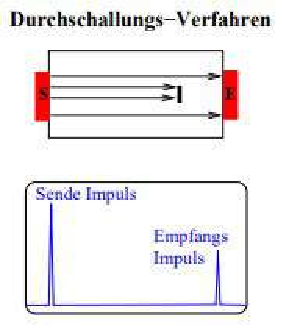
\includegraphics[width=\textwidth]{content/durchschall.pdf}
%    \caption{Das Durchschallungsverfahren skizziert. Durch die Pfeile kann bildlich nochvollzogen werden, warum so wenige Aussagen über die Fehlstelle getroffen werden können.\cite{anleitung}}
%    \label{fig:durchschall}
%\end{figure}

\subsubsection{Das Impuls-Echo-Verfahren}
\label{subsubsec:impuls-echo}
Hier ist der Ultraschallsender auch gleichzeitig der Empfänger.
Der kurze Impuls wird bei einer Grenzfläche reflektiert und wieder aufgenommen.
Aussagen über die Fehlstellen wie ihre Größe oder ihre Position können mithilfe der Höhe des Echos, der Schallgeschwindigkeit und der Laufzeit $t$ gemacht werden.
Es ergibt sich der Zusammenhang: 
\begin{equation} \label{eqn:schallgeschw}
    s = \frac{1}{2} c \cdot t
\end{equation}
In \autoref{fig:impuls-echo} wird dieses Prinzip der Reflexion anschaulich skizziert.

%\begin{figure}
%    \centering
%    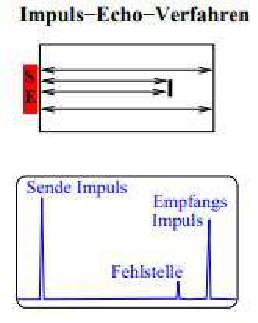
\includegraphics[width=\textwidth]{content/impuls_echo.pdf}
%    \caption{Das Impuls-Echo-Verfahren skizziert. Durch die aufgenommene Reflexion der Impulse können mehr Aussagen über die Fehlstelle getroffen werden. \cite{anleitung}}
%    \label{fig:impuls-echo}
%\end{figure}

\begin{figure}
    \begin{subfigure}{0.48\textwidth}
        \centering
        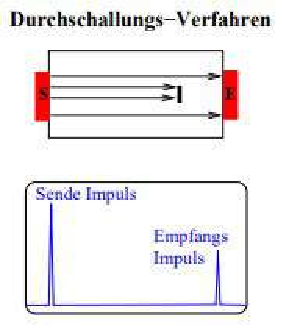
\includegraphics[height=5cm]{content/durchschall.pdf}
        \caption{Das Durchschallungsverfahren skizziert. Durch die Pfeile kann bildlich nochvollzogen 
                werden, warum so wenige Aussagen über die Fehlstelle getroffen werden können.\cite{anleitung}}
        \label{fig:durchschall}
    \end{subfigure}
\hfill 
    \begin{subfigure}{0.48\textwidth}
        \centering
        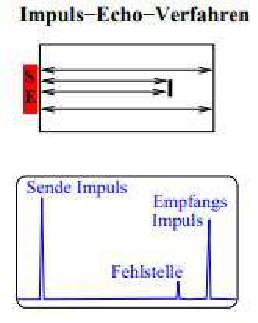
\includegraphics[height=5cm]{content/impuls_echo.pdf}
        \caption{Das Impuls-Echo-Verfahren skizziert. Durch die aufgenommene Reflexion der Impulse können mehr Aussagen über die Fehlstelle getroffen werden. \cite{anleitung}}
        \label{fig:impuls-echo}
    \end{subfigure}
    \caption{Die beiden Abbildunge zu den unterschiedlichen Messverfahren.}
    \label{fig:messmethoden}
\end{figure}